\section{Filtros}

Los \textbf{Filtros CSS} permiten agregar una capa de efectos gráficos, como desenfoque o cambio de color a un elemento, suelen ser utilizados estos filtros para ajustar el renderizado de imágenes, fondos y bordes. El filtrado de imágenes es útil cuando se requiere tener distintos estilos para una sola imagen; en vez de subir la misma imagen varias veces pero con distinta edición, se puede subir solamente una vez y aplicarle varios filtros con estilos distintos.

Los filtros no están disponibles para Internet Explorer, Edge 12, Safari 5.1 y versiones anteriores del mismo.

Por ejemplo, el método \textit{drop-shadow()} crea una sombra para un elemento, sus parámetros son:
\begin{center}
    \textit{filter: drop-shadow(width height blur color)}
\end{center}

Vemos que esta propiedad tiene los mismos parámetros que \textit{box-shadow}, a diferencia de que no incluye el parámetro \textit{spread}. La \textit{Figura \ref{fig: 57}} tiene el resultado de un ejemplo:
\begin{lstlisting}
estilos.css
    img {
        width: 130px;
        height: 100px;
    }
    /* Filtro de sombra con desenfoque. */
    .dropshadow {
        filter: drop-shadow(5px 9px 2px blue);
    }

prueba.html
    Image<br>
    <img src="http://www.sololearn.com/images/tree.jpg"/>
    <p>Drop Shadow 5px 9px 2px blue<p>
    <img class="dropshadow" src="http://www.sololearn.com/images/tree.jpg"/>
\end{lstlisting}
\begin{figure}[H]
    \centering
    \caption{Método \textbf{drop-shadow()} para agregar una sombra a un elemento}
    \label{fig: 57}
    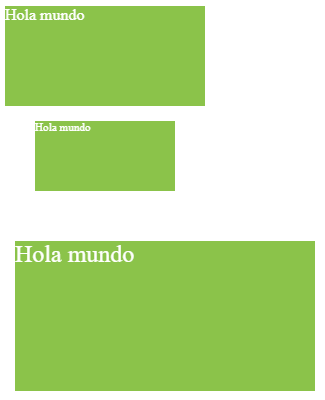
\includegraphics[width=5cm]{ss/scale.png}
\end{figure}


\subsection{Funciones}

Algunos de los métodos disponibles para los filtros son:
\begin{itemize}
    \item \textbf{blur()}: aplica un efecto de desenfoque a un elemento. Acepta un valor entero, no porcentajes, donde este valor es el radio de píxeles que se mezclan entre sí (un valor mayor crea mayor desenfoque). Si no se escribe un valor en el parámetro, el valor por defecto es 0.
    \item \textbf{brightness()}: ajusta el brillo de un elemento, haciendo que se vea más brillosa u oscura. 0\% es un elemento completamente oscuro, 100\% es un elemento sin cambio alguno y valores mayores al 100\% produce una imagen brillosa. Los valores enteros permitidos van de 0 a 1, cualquier valor negativo simplemente hará la imagen negra.
    \item \textbf{contrast()}: ajusta el contraste de un elemento. 0\% representa un elemento completamente gris, 100\% es el elemento sin cambios, entonces, el contraste se maneja entre valores mayores y menores al 100\%. Los valores enteros permitidos van de 0 a 1, cualquier valor negativo no aplicará un cambio al elemento.
    \item \textbf{drop-shadow()}.
    \item \textbf{grayscale()}: agrega una escala de grises a un elemento. El único parámetro disponible es el porcentaje o valor entero de la escala a aplicar, donde 0\% es el elemento original y 100\% tiene una escala de grises completa. Cualquier valor negativo no hará efecto en el elemento. Los valores enteros permitidos van de 0 a 1.
    \item \textbf{hue-rotate()}: aplica una rotación de tonos (basada en el círculo de colores presente en la \textit{Figura \ref{fig: 58}}) a un elemento. Este método recibe un ángulo como parámetro, 0 y 360 es el color rojo y lo puede ajustar como requiera.
    \item \textbf{invert()}: invierte los colores de un elemento de tal forma que se aplica brillo a zonas oscuras y se oscurecen zonas brillosas. La forma de trabajar este método es el mismo que \textit{grayscale}, sin embargo, acepta valores mayores al 100\%, pero estos no tendrán efecto en el elemento.
    \item \textbf{opacity()}: establece un efecto de transparencia a un elemento. 0\% es el valor para un elemento completamente transparente y 100\% es el elemento original. No acepta valores enteros.
    \item \textbf{saturate()}: controla la saturación de un elemento. El único parámetro disponible es el porcentaje o valor entero de la proporción de saturación a aplicar, donde 0\% es \textbf{completamente insaturada} (escala de grises) y 100\% es el elemento original. Los valores enteros permitidos van de 0 a 1.
    \item \textbf{sepia()}: convierte un elemento a sepia. La forma de trabajar este método es el mismo que \textit{grayscale}, sin embargo, acepta valores mayores al 100\%.
\end{itemize}
\begin{figure}[H]
    \centering
    \caption{El círculo de colores}
    \label{fig: 58}
    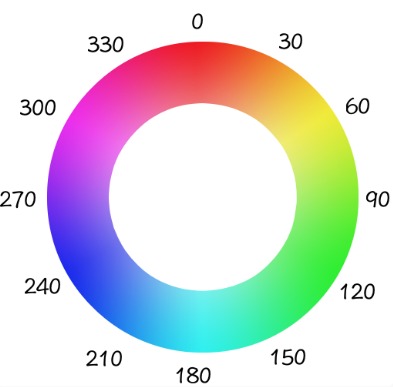
\includegraphics[width=5cm]{ss/circle-of-colors.png}
\end{figure}

Mostramos ejemplos de los métodos anteriormente mencionados en las \textit{Figuras \ref{fig: 59}} y \textit{\ref{fig: 60}} respectivamente:
\begin{lstlisting}
estilos.css
    /* Clase para mostrar contenedores uno al lado del otro. */
    .cont {
        display: inline-block;
    }
    /* Clase para contener etiqueta e imagen. */
    .layout {
        display: inherit;
    }
    /* Filtro de escala de grises, rotación de tonos, inversión, saturación y sepia. */
    .grayscale {
        filter: grayscale(100%);
    }
    .hue-rotate {
        filter: hue-rotate(180deg);
    }
    .invert {
        filter: invert(70%);
    }
    .saturate {
        filter: saturate(25%);
    }
    .sepia {
        filter: sepia(70%);
    }

prueba.html
    <div class="cont">
        <div class="layout">
            <p>Original</p>
            <img src="http://www.sololearn.com/images/tree.jpg" alt="">
        </div>
        <div class="layout">
            <p>Grayscale</p>
            <img src="http://www.sololearn.com/images/tree.jpg" alt="" class="grayscale">
        </div>
        <div class="layout">
            <p>Hue-rotate</p>
            <img src="http://www.sololearn.com/images/tree.jpg" alt="" class="hue-rotate">
        </div>
        <div class="layout">
            <p>Invert</p>
            <img src="http://www.sololearn.com/images/tree.jpg" alt="" class="invert">
        </div>
        <div class="layout">
            <p>Saturate</p>
            <img src="http://www.sololearn.com/images/tree.jpg" alt="" class="saturate">
        </div>
        <div class="layout">
            <p>Sepia</p>
            <img src="http://www.sololearn.com/images/tree.jpg" alt="" class="sepia">
        </div>
    </div>
\end{lstlisting}
\begin{figure}[H]
    \centering
    \caption{Conjunto 1 de ejemplos de filtros CSS}
    \label{fig: 59}
    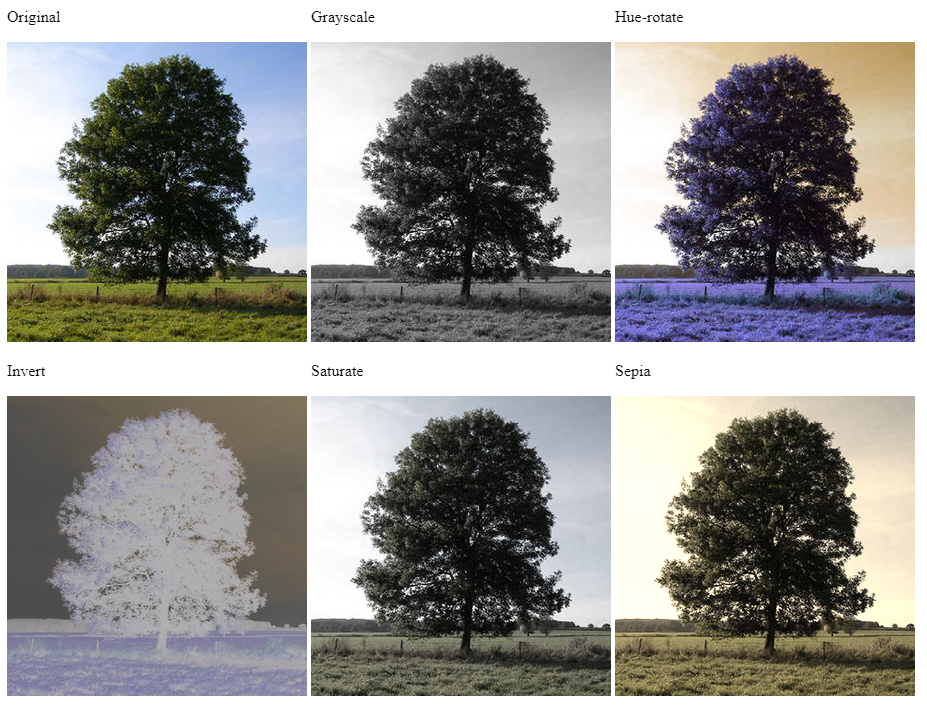
\includegraphics[width=14cm]{ss/filter-examples-1.png}
\end{figure}
\begin{lstlisting}
estilos.css
    /* Clase para mostrar contenedores uno al lado del otro. */
    .cont {
        display: inline-block;
    }
    /* Clase para contener etiqueta e imagen. */
    .layout {
        display: inherit;
    }
    /* Filtros de opacidad, brillo, contraste y desenfoque. */
    .opacity {
        filter: opacity(70%);
    }
    .brightness {
        filter: brightness(50%);
    }
    .contrast {
        filter: contrast(140%);
    }
    .blur {
        filter: blur(10px);
    }

prueba.html
    <div class="cont">
        <div class="layout">
            <p>Original</p>
            <img src="http://www.sololearn.com/images/tree.jpg" alt="">
        </div>
        <div class="layout">
            <p>Opacity</p>
            <img src="http://www.sololearn.com/images/tree.jpg" alt="" class="opacity">
        </div>
        <div class="layout">
            <p>Brightness</p>
            <img src="http://www.sololearn.com/images/tree.jpg" alt="" class="brightness">
        </div>
        <div class="layout">
            <p>Contrast</p>
            <img src="http://www.sololearn.com/images/tree.jpg" alt="" class="contrast">
        </div>
        <div class="layout">
            <p>Blur</p>
            <img src="http://www.sololearn.com/images/tree.jpg" alt="" class="blur">
        </div>
    </div>
\end{lstlisting}
\begin{figure}[H]
    \centering
    \caption{Conjunto 2 de ejemplos de filtros CSS}
    \label{fig: 60}
    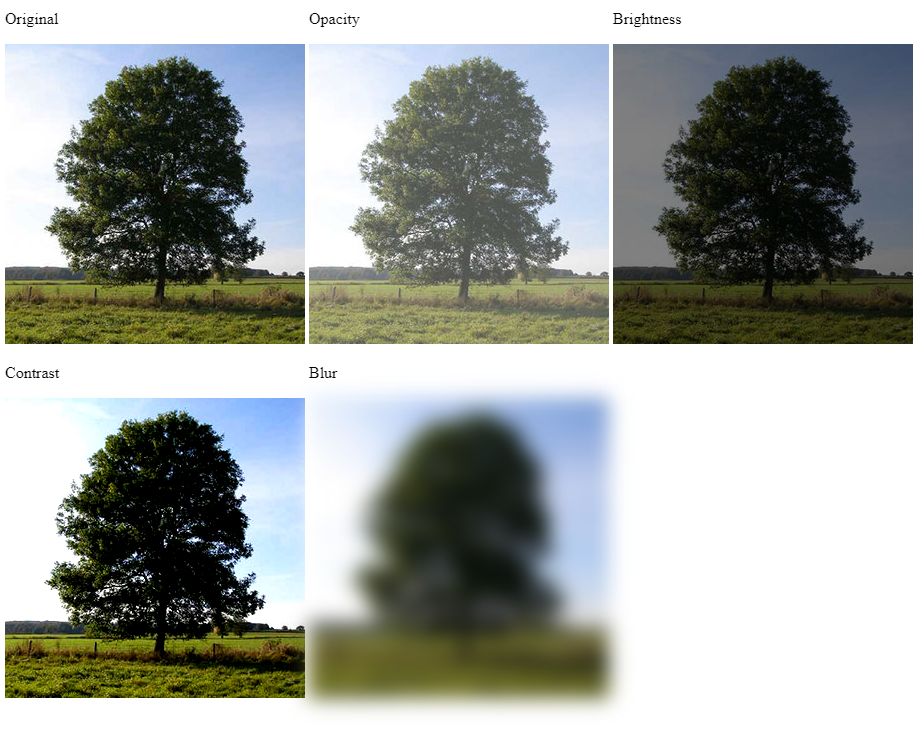
\includegraphics[width=14cm]{ss/filter-examples-2.png}
\end{figure}


\subsection{Usando múltiples filtros}

Se pueden aplicar varios estilos a un solo elemento, simplemente se separan por espacios, como se ve en la \textit{Figura \ref{fig: 61}}:
\begin{lstlisting}
estilos.css
    .filtered {
        /* Agrega filtros de saturación, sombra y desenfoque. */
        filter: saturate(30%) drop-shadow(5px 9px 2px gray) blur(1px);
    }

prueba.html
    <img class="original" src="http://www.sololearn.com/images/tree.jpg">
    <img class="filtered" src="http://www.sololearn.com/images/tree.jpg">
\end{lstlisting}
\begin{figure}[H]
    \centering
    \caption{Uso de múltiples filtros CSS}
    \label{fig: 61}
    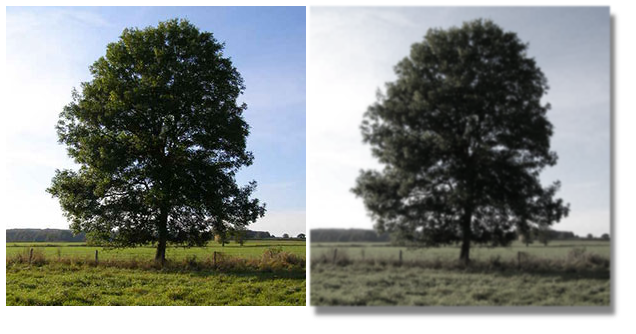
\includegraphics[width=10cm]{ss/filter-multiple.png}
\end{figure}
